\subsection{Low concentrations of phosphatidylethanolamine} 
	
	Because phosphatidylethanolamine isn't a reported component of the 42-Max-UB-medium, $Tabla\ 1$, and it can be a carbon source for the $GEMs$, its concentration was set first to the lowest value possible. For $Recon3D$ it was fixed to 0.5mM (a handpicked value) and for $CHO$ it wasn't present in the feed medium at all.
	
		\begin{figure}[H]
		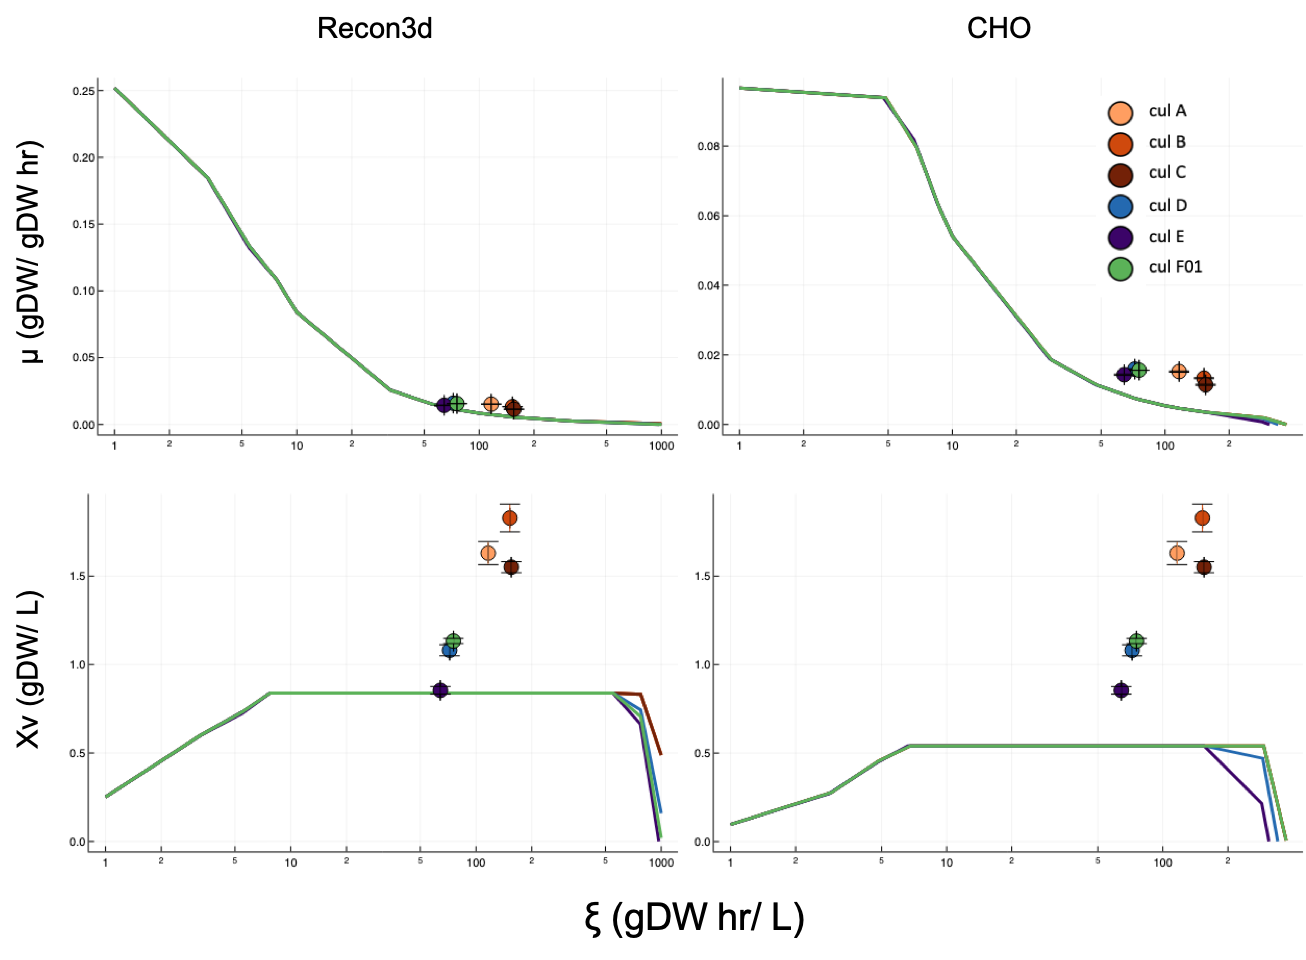
\includegraphics[scale = 0.5]{low_medium_1}
		\caption{$FBA$ results showing the growth rate, $\mu$, and the viable cell density, $Xv$, dependence of $\xi$ for the six steady states. The solid lines represent the model predictions and the colored points show the experimental results. The model data was obtained for feed mediums with 0.5mM ($Recon3D$) and 0.0mM ($CHO$) concentration of phosphatidylethanolamine}
		
	\end{figure}
	
	Flux balance analysis with molecular crowding (FBA) was performed similarly to \shortcite{Fernandez-de-Cossio-Diaz2018b}. Plots of $\mu$ and $Xv$ as a function of $\xi$ are shown in $Figure\ 1$. Both networks failed to reach the experimental values for both observables. In the case of $Xv$, in all the explored $\xi$ range (from 1 to 1000 gDW hr/ L) the value was underestimated. This result may have several causes. One could be that the $GEM$ has a "too expensive" biomass equation. We mean that one or more biomass required precursors might be overestimated. However, this reason seems hard to sustain because we modified the $Recon3D$ biomass equation with the reported anabolic biomass demand for AGE1.HN.AA1 \shortcite{Niklas2013}. We used the reported anabolic demand of proteins, lipids, DNA, RNA, and carbohydrates to fix the total demand of these same groups in the original $Recon3D$ biomass equation. For $CHO$ we kept the biomass equation unmodified. Nonetheless, a modification in the biomass equation would be an elegant way to solve the problem. Another plausible cause could be a big difference between the model's frameworks. But, both works model the chemostat in an equivalent fashion, as can be seen when comparing equations 1 with 3.25, and 2 with 3.28 and 3.29, from \shortcite{Fernandez-de-Cossio-Diaz2017} and \shortcite{Rath2017a} respectively.
	 
		\begin{figure}[H]
		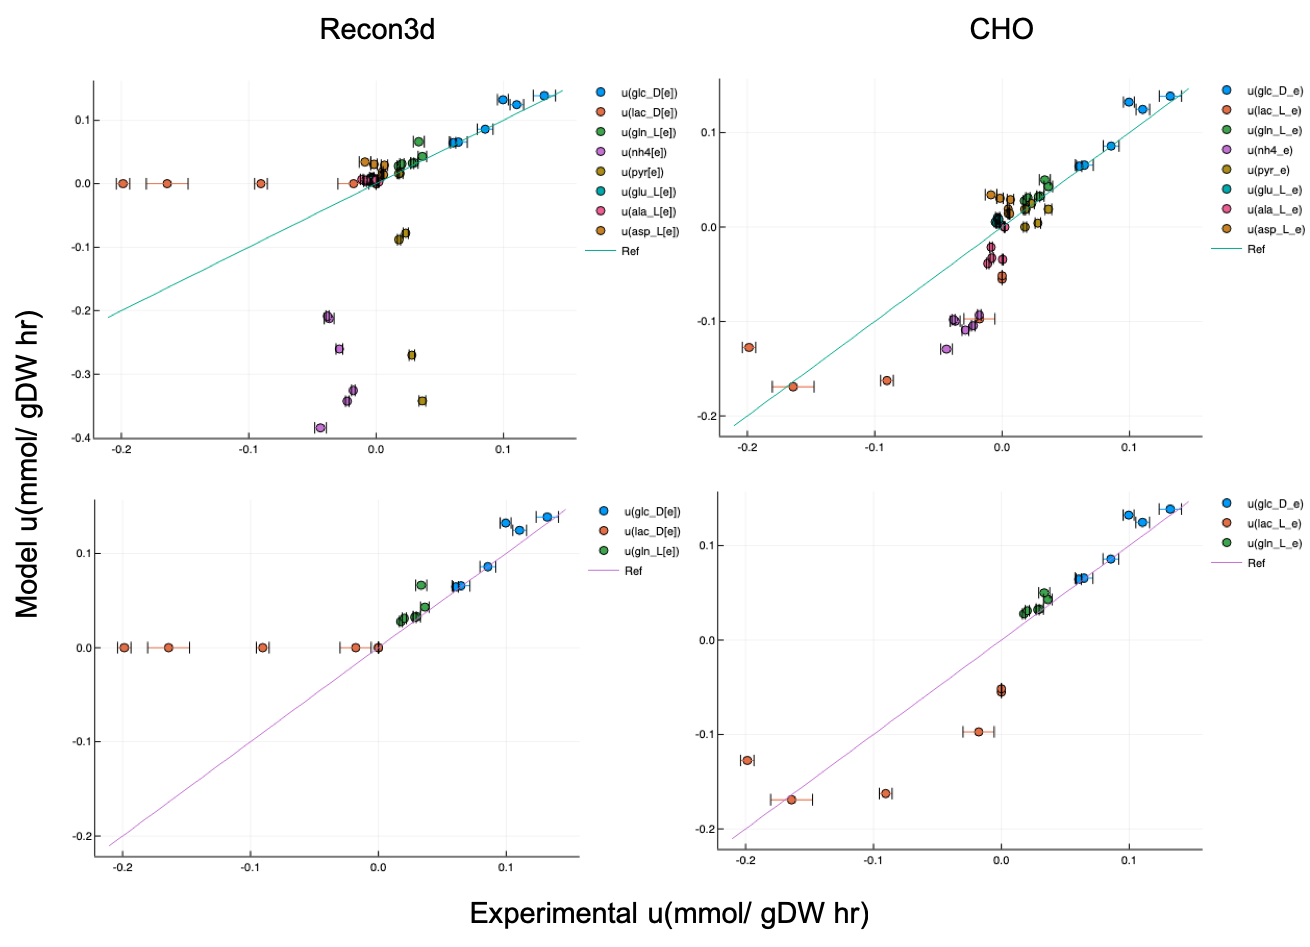
\includegraphics[scale = 0.5]{low_medium_2}
		\caption{Correlations of all the experimental uptakes, upper graphs, and a selected subset, inferior graphs, respect to the predicted value from $FBA$ with 0.5mM ($Recon3D$) and 0.0mM ($CHO$) concentration of phosphatidylethanolamine.}
		
	\end{figure}
	
	Moreover, other parameter than can affect $Xv$ is the bleeding coefficient, $\phi$,
	defined in perfusion systems as the fraction of cells that escape from the culture through a cell-retention device \shortcite{Fernandez-de-Cossio-Diaz2017}. Because, \shortcite{Rath2017a} doesn't report the use of any retention devise in the cultures this parameter was taken as 1.0, but lower values will cause to increment the predicted value of  $Xv$ by the model. Finally, it needs to be taken into consideration that we are using $GEMs$ that are not directed curated for the working cell line. In fact, a crucial phenotypic feature reported for AGE1.HN.AA1 like the impossibility of growth in $GLN$ free mediums \shortcite{Rath2017a} is not reproduced by the used $GEMs$. This is, by far, the most difficult factor to solve, because the curation of a genome-scale metabolic network is a very laborious process.

	
	On the other hand, correlations of experimental and modeled uptakes, $Figure\ 2$, were performed. The graphs show better results for the uptakes of $GLC$ and $GLN$, 
	and worse correlations for uptakes such as $PYR$, $NH4$ and $LAC$ for both $GEMs$. In general, $CHO$ had better correlations than $Recon3D$. This could be, maybe, explained because $Recon3D$ is a general $GEM$, allowing the model to access to all the human genome repertory, a fact that is not accurate for a cell in the $in\ vivo$ scenario. Additionally, $CHO$ was curated for a defined cell line, representing a more restricted and realistic network. Anyway, it is remarkable that the models reproduce uptakes like $GLC$ and $GLN$ regarding all the previous consideration.